\documentclass[tikz,border=5pt]{standalone}

\usepackage{amsmath, amssymb, tikz} % Required for mathematical symbols and formatting
\usetikzlibrary{positioning, backgrounds, calc, }

\begin{document}


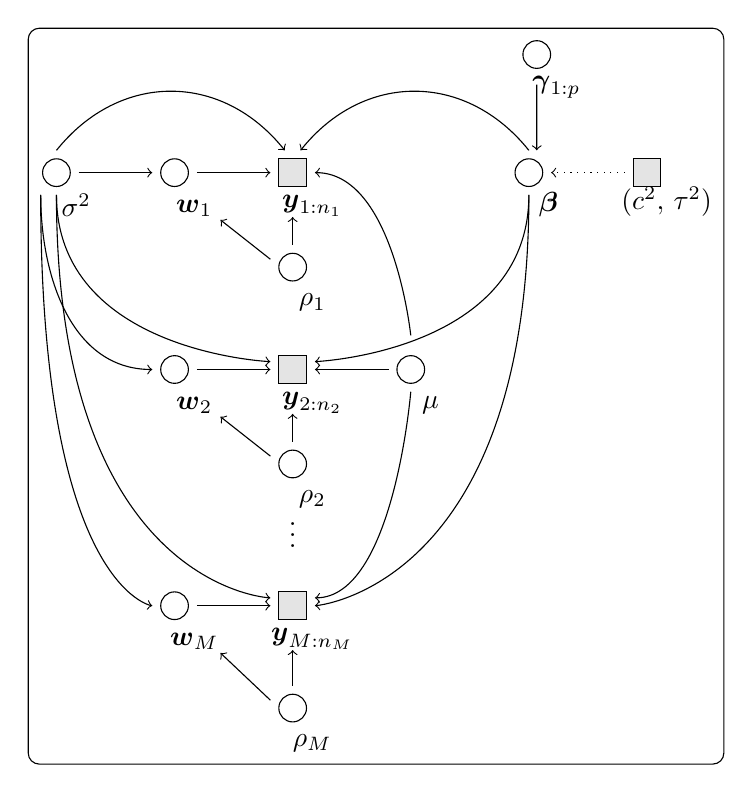
\begin{tikzpicture}[every node/.style={inner sep=0}, framed, background rectangle/.style={draw=black, rounded corners}]


% \draw[very thin, gray] (-5, -5) grid (5, 5);
% % Add axis labels
% \foreach \x in {-1,...,5}
% \draw[gray] (\x,-3) -- (\x,-3.2) node[below] {\tiny \x};
% \foreach \y in {-5,...,5}
% \draw[gray] (-1,\y) -- (-1.2,\y) node[left] {\tiny \y};

% \node[right, circle, draw]

\node[circle, draw,  fill=white, inner sep=0pt, minimum size=10pt, label={[xshift=0.25cm, yshift=-0.75cm]$\sigma^{2}$}] (sigma2) at (-4, 4) {};

\node[circle, draw,  fill=white, inner sep=0pt, minimum size=10pt, label={[xshift=0.25cm, yshift=-0.75cm]$\boldsymbol{w}_{1}$}] (w1) at (-2.5, 4) {};

\node[rectangle, draw, fill=gray!70!white!30, inner sep=0pt, minimum size=10pt, label={[xshift=.25cm, yshift=-0.75cm]$\boldsymbol{y}_{1:n_{1}}$}] (y1) at (-1, 4) {};

% \node[circle, draw,  fill=white, inner sep=0pt, minimum size=10pt, label={[xshift=0.25cm, yshift=-0.75cm]$\mu_{1}$}] (mu1) at (0.5, 4) {};

\node[circle, draw, label={[xshift=0.25cm, yshift=-0.75cm]$\rho_{1}$}, minimum size=10pt, inner sep=0pt] (rho1) at (-1, 2.8) {};

\node[circle, draw,  fill=white, inner sep=0pt, minimum size=10pt, label={[xshift=0.25cm, yshift=-0.75cm]$\boldsymbol{w}_{2}$}] (w2) at (-2.5, 1.5) {};

\node[rectangle, draw, fill=gray!70!white!30, inner sep=0pt, minimum size=10pt, label={[xshift=.25cm, yshift=-0.75cm]$\boldsymbol{y}_{2:n_{2}}$}] (y2) at (-1, 1.5) {};

% era mu2, ahora solo considero un mu
% \node[circle, draw,  fill=white, inner sep=0pt, minimum size=10pt, label={[xshift=0.25cm, yshift=-0.75cm]$\mu_{2}$}] (mu2) at (0.5, 1.5) {};
\node[circle, draw,  fill=white, inner sep=0pt, minimum size=10pt, label={[xshift=0.25cm, yshift=-0.75cm]$\mu$}] (mu) at (0.5, 1.5) {};

\node[circle, draw, label={[xshift=0.25cm, yshift=-0.75cm]$\rho_{2}$}, minimum size=10pt, inner sep=0pt] (rho2) at (-1, 0.3) {};

\node[] (y3) at (-1, -0.5) {$\vdots$};

\node[circle, draw,  fill=white, inner sep=0pt, minimum size=10pt, label={[xshift=0.25cm, yshift=-0.75cm]$\boldsymbol{w}_{M}$}] (wM) at (-2.5, -1.5) {};

\node[rectangle, draw, fill=gray!70!white!30, inner sep=0pt, minimum size=10pt, label={[xshift=.25cm, yshift=-0.75cm]$\boldsymbol{y}_{M:n_{M}}$}] (yM) at (-1, -1.5) {};

% \node[circle, draw,  fill=white, inner sep=0pt, minimum size=10pt, label={[xshift=0.25cm, yshift=-0.75cm]$\mu_{M}$}] (muM) at (0.5, -1.5) {};

\node[circle, draw, label={[xshift=0.25cm, yshift=-0.75cm]$\rho_{M}$}, minimum size=10pt, inner sep=0pt] (rhoM) at (-1, -2.8) {};

\node[circle, draw,  fill=white, inner sep=0pt, minimum size=10pt, label={[xshift=0.25cm, yshift=-0.75cm]$\boldsymbol{\beta}$}] (beta) at (2, 4) {};

\node[circle, draw,  fill=white, inner sep=0pt, minimum size=10pt, label={[xshift=0.25cm, yshift=-0.75cm]$\boldsymbol{\gamma}_{1:p}$}] (gammabeta) at (2.1, 5.5) {};

\node[rectangle, draw,  fill=gray!70!white!30, inner sep=0pt, minimum size=10pt, label={[xshift=0.25cm, yshift=-0.75cm]$(c^{2},\, \tau^{2})$}] (hyperbeta) at (3.5, 4) {};

% \node[circle, draw,  fill=white, inner sep=0pt, minimum size=10pt, label={[xshift=0.25cm, yshift=-0.75cm]$\boldsymbol{\gamma}_{1:M}$}] (gammamu) at (2.1, -1.5) {};

% \node[circle, draw,  fill=white, inner sep=0pt, minimum size=10pt, label={[xshift=0.25cm, yshift=-0.75cm]$(\mu_{0},\, \sigma^{2}_{\mu})$}] (muprior) at (2.1, -1.5) {};


% sigma2 a wi
% \draw[->, dotted]
\draw[->] ([xshift=1mm]sigma2.east) -- ([xshift=-1mm]w1.west);
\draw[->] ([xshift=-2mm, yshift=-1mm]sigma2.south) to[out=-90, in=180] ([xshift=-1mm]w2.west);
% ...
% \draw[->] (sigma2.south) |- (w2.west);
% \draw[->] ([xshift=0mm]sigma2.south) to[out=270, in=180] ([xshift=0mm]wM.west);
% \draw[->] (sigma2.south) to[bend right=25] (wM.west);
\draw[->] ([yshift=-1mm, xshift=-2mm]sigma2.south) .. controls +(0, -5) and +(0, 0) .. ([xshift=-1mm, yshift=0mm]wM.west);

% wi a yi
\draw[->] ([xshift=1mm]w1.east) -- ([xshift=-1mm]y1.west);
\draw[->] ([xshift=1mm]w2.east) -- ([xshift=-1mm]y2.west);
% ...
\draw[->] ([xshift=1mm, yshift=0mm]wM.east) -- ([xshift=-1mm, yshift=0mm]yM.west);

% rhoi a yi
\draw[->] ([yshift=1mm]rho1.north) -- ([yshift=-3.8mm]y1.south);
\draw[->] ([yshift=1mm]rho2.north) -- ([yshift=-3.8mm]y2.south);
% ...
\draw[->] ([yshift=1mm]rhoM.north) -- ([yshift=-3.8mm]yM.south);

% mui a yi
% unico mu:
\draw[<-] ([xshift=1mm]y1.east) .. controls +(1, 0) and +(0, 0) .. ([xshift=0mm, yshift=2.5mm]mu.north);
% ...
\draw[<-] ([xshift=1mm]y2.east) -- ([xshift=-1mm]mu.west);
\draw[<-] ([xshift=1mm, yshift=1mm]yM.east) .. controls +(1, 0) and +(0, 0) .. ([xshift=0mm, yshift=-1mm]mu.south);
%
% \draw[<-] ([xshift=1mm]y1.east) -- ([xshift=-1mm]mu1.west);
% \draw[<-] ([xshift=1mm]y2.east) -- ([xshift=-1mm]mu2.west);
% ...
% \draw[<-] ([xshift=1mm]yM.east) -- ([xshift=-1mm]muM.west);

% rhoi a wi
\draw[->] ([xshift=-1mm, yshift=1mm]rho1.west) -- ([xshift=4mm, yshift=-6mm]w1.east);
\draw[->] ([xshift=-1mm, yshift=1mm]rho2.west) -- ([xshift=4mm, yshift=-6mm]w2.east);
% ...
\draw[->] ([xshift=-1mm, yshift=1mm]rhoM.west) -- ([xshift=4mm, yshift=-6mm]wM.east);

% sigma2 a yi
\draw[->] ([yshift=1mm]sigma2.north) .. controls +(0.8, 1) and +(-0.8, 1) .. ([xshift=-1mm, yshift=1mm]y1.north);
\draw[->] ([yshift=-1mm, xshift=0mm]sigma2.south) .. controls +(0, -2) and +(0, 0) .. ([xshift=-1mm, yshift=1mm]y2.west);
% ...
\draw[->] ([yshift=-1mm, xshift=0mm]sigma2.south) .. controls +(0, -5) and +(0, 0) .. ([xshift=-1mm, yshift=1mm]yM.west);

% beta a yi
\draw[->] ([yshift=1mm]beta.north) .. controls +(-0.8, 1) and +(0.8, 1) .. ([xshift=1mm, yshift=1mm]y1.north);
\draw[->] ([yshift=-1mm]beta.south) .. controls +(0, -2) and +(0, 0) .. ([xshift=1mm, yshift=1mm]y2.east);
% ...
\draw[->] ([yshift=-1mm]beta.south) .. controls +(0, -5) and +(0, 0) .. ([xshift=1mm, yshift=0mm]yM.east);

% gamma mu a mui
% ahora son muprior a mu
% \draw[->, dotted] ([xshift=-1mm]muprior.west) -- ([xshift=1mm]muM.east) ;
%% \draw[->] ([xshift=0mm, yshift=1mm]muprior.north) -- ([xshift=4mm, yshift=-4.4mm]mu2.south) ;
% \draw[->, dotted] ([xshift=0mm, yshift=1mm]muprior.north) to[out=90, in=0] ([xshift=1mm, yshift=0mm]mu2.east) ;
...
% \draw[->, dotted] ([yshift=1mm]muprior.north) .. controls +(0, 5) and +(0, 0) .. ([xshift=1mm, yshift=0mm]mu1.east);

% gamma beta a beta
\draw[->] ([yshift=-2mm]gammabeta.south) -- ([xshift=1mm, yshift=1mm]beta.north) ;

% hyperbeta a beta
\draw[->, dotted] ([xshift=-1mm, yshift=-0mm]hyperbeta.west) -- ([xshift=1mm, yshift=0mm]beta.east) ;

\end{tikzpicture}


\end{document}

https://tex.stackexchange.com/questions/471690/elbow-arrow-between-two-nodes

https://tex.stackexchange.com/questions/58878/tikz-set-node-label-position-more-precisely